\documentclass[fleqn]{scrartcl}% fleqn aligns math equations to the left

\usepackage[T1]{fontenc}%
\usepackage[utf8]{inputenc}%
\usepackage{lmodern}%
\usepackage{textcomp}%
\usepackage{lastpage}%
\usepackage{parskip}%
\usepackage[letterpaper,left=0.8in, right=0.75in, top=1.0in, bottom=0.75in, includefoot, heightrounded]{geometry}%
\usepackage{graphicx}%
\usepackage{amsmath}
\usepackage[hidelinks]{hyperref}%
\usepackage{blindtext}
\usepackage[super]{natbib} % for references in superscript

% note: we are preficing figures with an S character 
\renewcommand\thefigure{S\arabic{figure}}


% submission requirements in ancient journals
\usepackage{lineno} % enumerate each line
\linenumbers
\linespread{2}
%%%%%%%%%%%%%%%%%%%%%%%%%%%%%%%%%%%%%%%%%%%%

\newcommand{\etal}{\textit{\!et al.\,}}


\title{Lorem ipsum dolor sit amet - supplementary material}%
\author{Marcus Tullius Cicero}%
\date{\today}%
%
\begin{document}

    \maketitle
    \begin{abstract}
        A result that does not use the ``novel\("\) word in its abstract.
    \end{abstract}


    \clearpage
    \section*{Introduction}
    Marcus Tullius Cicero  - supplementary blah blah.

    \clearpage
    \section*{Suppl Methods}
    \blindtext




    \clearpage
    \section*{Suppl Discussion}
    \blindtext


    \clearpage
    \bibliography{cicero}


    \clearpage
    \section*{Figures}

    \begin{figure}[ht]%
        % note: figure argument should not include the extension
        \centering{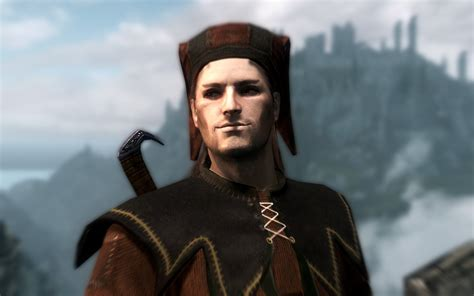
\includegraphics[width=0.5\linewidth]{figures/cicero-skyrim}}
        \caption {Cicero, Skyrim version.}
        \label{fig:ciceroskyrim} % referenced in the main document
    \end{figure}





\end{document}